\documentclass[a4paper]{article}

\usepackage[english]{babel}
\usepackage[utf8]{inputenc}
\usepackage{amsmath}
\usepackage{graphicx}
\usepackage[colorinlistoftodos]{todonotes}
\usepackage{xeCJK}
\usepackage{abstract}


\title{海狮识别}

\author{第八组}

\date{\today}

\begin{document}
\maketitle

\renewcommand{\abstractname}{摘要}
\begin{onecolabstract}
Enter a short summary here. What topic did you want to investigate and why? What experiment did you perform? What were your main results and conclusion?
\end{onecolabstract}

\section{题目描述}
\label{sec:introduction}

Write a short introduction about what you did in the lab.

Briefly explain what methods you will use in the experiment, and what values you will extract from the data.

If you want to cite something you can do it like this\cite{nano3}, this will refer to the medium defined in the end that has the tag nano3.

\section{背景}
\label{sec:theory}

\subsection{this is how you make a subsection}
No theory really needed for this experiment.

\section{解决思路}

\subsection{Experimental set-up}
Explain the experimental set-up here. Use a schematic picture (make it yourself in photoshop, paint, powerpoint (powerpoint is very underrated for quick drawings)) to show how the components are connected. Briefly explain how a lock-in amplifier works.

\section{结果}

\subsection{Resistor}


Show the 2 graphs for transistor behavior as asked for in the manual.

\begin{figure}
\centering
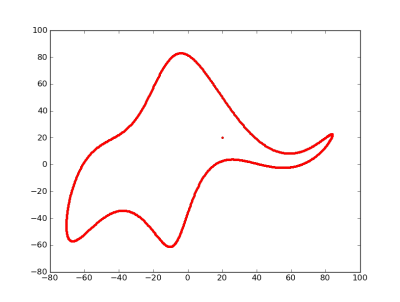
\includegraphics[width=1\textwidth]{elephant.png}
\caption{\label{fig:data1}Replace this figure \cite{elephant} with the one you've made and add an appropriate caption. }
\end{figure}

\subsection{Transistor}
Include the two 2D plots you made about the behavior of the resistor. Most of the time \LaTeX doesn't put the figures where you would expect them but where they are ideally place from a layout prospective, you can always just refer to the number of the picture with the label command for example Figure \ref{fig:data}.

\begin{figure}
\centering
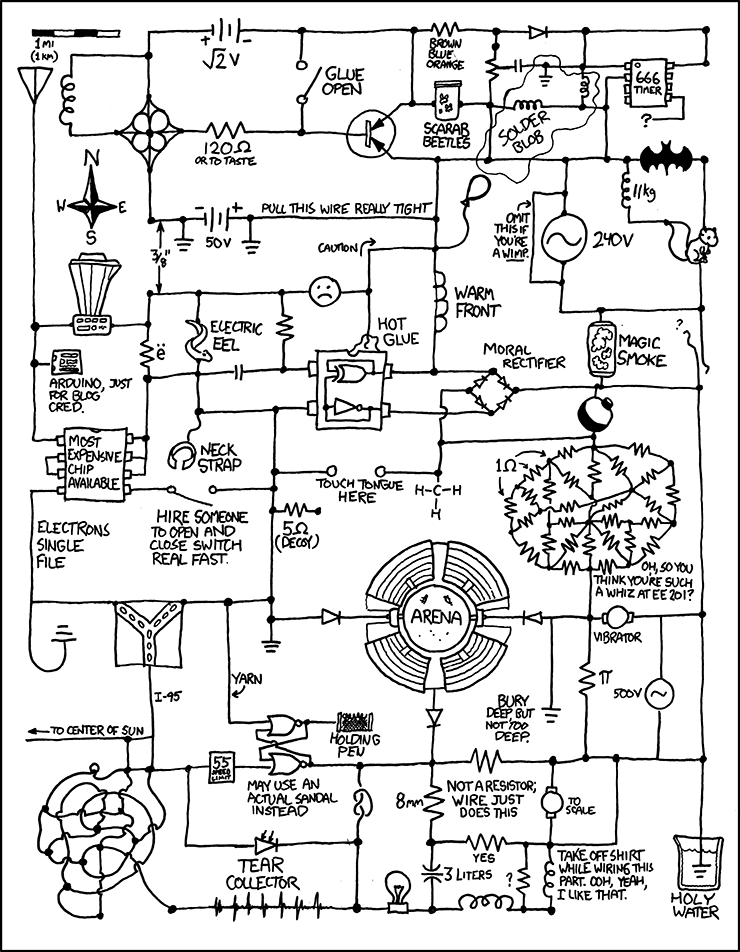
\includegraphics[width=0.5\textwidth]{circuit_diagram.png}
\caption{\label{fig:data}Replace this figure  \cite{xkcd} with the one you've made and add an appropriate caption. By the way you should always cite when you put any stuff in your reports you didn't make yourself.}
\end{figure}



\newpage
\section{Some LaTeX tips}
\label{sec:latex}
\subsection{How to Include Figures}

First you have to upload the image file (JPEG, PNG or PDF) from your computer to writeLaTeX using the upload link the project menu. Then use the includegraphics command to include it in your document. Use the figure environment and the caption command to add a number and a caption to your figure. See the code for Figure \ref{fig:frog} in this section for an example.

\begin{figure}
\centering

\includegraphics[width=0.3\textwidth]{frog.jpg}
\caption{\label{fig:frog}This frog was uploaded to writeLaTeX via the project menu.}
\end{figure}

\subsection{How to Make Tables}

Use the table and tabular commands for basic tables --- see Table~\ref{tab:widgets}, for example.

\begin{table}
\centering
\begin{tabular}{l|r}
Item & Quantity \\\hline
Widgets & 42 \\
Gadgets & 13
\end{tabular}
\caption{\label{tab:widgets}An example table.}
\end{table}

\subsection{How to Write Mathematics}

\LaTeX{} is great at typesetting mathematics. Let $X_1, X_2, \ldots, X_n$ be a sequence of independent and identically distributed random variables with $\text{E}[X_i] = \mu$ and $\text{Var}[X_i] = \sigma^2 < \infty$, and let

\begin{equation}
S_n = \frac{X_1 + X_2 + \cdots + X_n}{n}
      = \frac{1}{n}\sum_{i}^{n} X_i
\label{eq:sn}
\end{equation}

denote their mean. Then as $n$ approaches infinity, the random variables $\sqrt{n}(S_n - \mu)$ converge in distribution to a normal $\mathcal{N}(0, \sigma^2)$.

The equation \ref{eq:sn} is very nice.

\subsection{How to Make Sections and Subsections}

Use section and subsection commands to organize your document. \LaTeX{} handles all the formatting and numbering automatically. Use ref and label commands for cross-references.

\subsection{How to Make Lists}

You can make lists with automatic numbering \dots

\begin{enumerate}
\item Like this,
\item and like this.
\end{enumerate}
\dots or bullet points \dots
\begin{itemize}
\item Like this,
\item and like this.
\end{itemize}
\dots or with words and descriptions \dots
\begin{description}
\item[Word] Definition
\item[Concept] Explanation
\item[Idea] Text
\end{description}

We hope you find write\LaTeX\ useful, and please let us know if you have any feedback using the help menu above.

\begin{thebibliography}{9}
\bibitem{nano3}
  K. Grove-Rasmussen og Jesper Nygård,
  \emph{Kvantefænomener i Nanosystemer.
  Niels Bohr Institute \& Nano-Science Center, Københavns Universitet}

\bibitem{elephant}
  How to fit an elephant,
  \emph{https://www.johndcook.com/blog/2011/06/21/how-to-fit-an-elephant/}
  
\bibitem{xkcd}
  xkcd 730,
  \emph{https://xkcd.com/730/}

\end{thebibliography}
\end{document}